\begin{center}
    
\includegraphics[width=1in]{bell.jpg}
\end{center}
\vspace{5ex}

Evaluate the function $f(x) = -x+2$ at $x=-1$

\vspace{15ex}

Fill out the table and plot $f(x)$

\begin{minipage}{0.3\textwidth}
\Large
\begin{tabular}{|c|c|}
\hline
    $x$ & $f(x)$  \\
    \hline \hline
    -1 &  \\
    \hline
    0 & \\
    \hline
    1 & \\
    \hline
    2 & \\
    \hline
\end{tabular}
\end{minipage}
\begin{minipage}{0.68\textwidth}
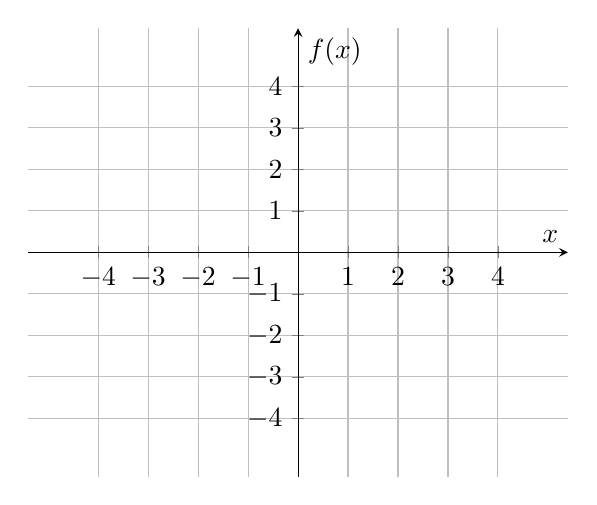
\begin{tikzpicture}
\begin{axis}[axis lines = middle,
            xlabel = $x$, ylabel = $f(x)$,
            domain=-4:4,
            samples=200,
            ymin=-4.5, ymax=4.5,
            xmin=-4.5, xmax=4.5,
            grid=both,
            xtick={-4,-3,-2,-1,1,2,3,4},
            ytick={-4,-3,-2,-1,1,2,3,4},
            enlargelimits=true]
\end{axis}
\end{tikzpicture}
\end{minipage}

\fancyfoot[OC,EC]{FLIP OVER}